\documentclass[11pt, reqno]{amsart} \usepackage{pstricks} % needed to make the mathematics subject classification show
\usepackage[authoryear]{natbib}

\usepackage[all,arc]{xy}
\usepackage{enumerate}
\usepackage{mathrsfs}
\usepackage{float}
\usepackage{amsmath}
\usepackage{amsthm}
\usepackage{amsfonts}
\usepackage{amssymb}
\usepackage{amsbsy}
\usepackage{graphicx}
\usepackage{enumitem}
\usepackage{physics}
\usepackage{bbm}
\usepackage{bm}
\usepackage[colorlinks, citecolor=blue, linkbordercolor={0 0 1}]{hyperref}
%% python
\usepackage{pythonhighlight}
\usepackage{pygmentex}
\lstnewenvironment{PythonA}[1][]{\lstset{style=mypython, #1}}{}
\lstnewenvironment{PythonB}[1][]{\lstset{style=mypython, frame=none, #1}}{}
\lstdefinestyle{Py2}{
  style=mypython,
  frame=none
  }

\newenvironment{nouppercase}{%
  \let\uppercase\relax%
  \renewcommand{\uppercasenonmath}[1]{}}{}
% style 
\newcommand{\pkg}[1]{{\fontseries{m}\fontseries{b}\selectfont #1}}
\let\proglang=\textsf
\def\@codex#1{{\normalfont\ttfamily\hyphenchar\font=-1 #1}\egroup}
\let\code=\texttt
% \ifx\csname urlstyle\endcsname\relax
%   \newcommand\@doi[1]{doi:\discretionary{}{}{}#1}\else
%   \newcommand\@doi{doi:\discretionary{}{}{}\begingroup
% \urlstyle{tt}\Url}\fi

\begin{document}

\title[Title]{\large
\pkg{RlassoModels}: Rigorous Lasso for High-Dimensional Estimation and Inference in \proglang{Python}}
\author{Matias Piqueras}


\begin{nouppercase}
\maketitle
\end{nouppercase}

\begin{abstract}
The \pkg{RlassoModels} package is a \proglang{Python} implementation of  
\end{abstract}


\section{Introduction}
\label{sec:intro}

The ever-increasing availability to data and computing power is fundamentally
reshaping empirical social scientific research. Instead of costly surveys,
political scientists can now leverage easily accessible social media data to
make point-estimates of ideology \citep{Barbera2015}. Sociologists, are able to
learn about the dynamics of large scale social networks and extract meaning
from text corpuses that would take more than a lifetime to read
\citep{Sapiezynski2019, Kozlowski2019}. In the field of economics, fundamental
but difficult to empirically identify concepts, such as demand curves can be
studied by using data of individual level transactions measured at an
unprecedented scale \citep{Cohen2016}. 

New data has also necessitated the use of new methods. The desirable asymptotic
properties of traditional statistical methods such as ordinary least squares
(OLS) implicitly assume and indeed require, that the amount of variables $p$ is
fixed as $n \to \infty$. This is most evidently seen in the expected prediction
error given by $E\left[\frac{1}{n} \sum_{i=1}^{n}\left(x_{i}^{\prime}
\hat{\beta}-x_{i}^{\prime} \beta\right)^{2}\right]=\frac{\sigma^{2} p}{n}$.
However, in many modern practical applications the data is high-dimensional, in
the $p>n$ or even $p \gg n$ sense, whereby the fraction $\frac{p}{n}$ is
nonnegliable and traditional methods badly behaved. To overcome this,
researchers have turned their attention to machine learning models such as tree
based learners and neural networks that are better attuned to this setting. In
\citep{Breiman2001} the tree based lear


\section{Related Software}

\pkg{lassopack} implements Lasso with data-driven and theoretically motivated
penalty in \proglang{Stata} \citep{Ahrens2020}. The extension \pkg{pdslasso}
implements the post-double-selection and post-regularization methodology for
inference in the presence of high-dimensional controls and/or instrumental
variables \citep{Ahrens2019}. In \proglang{R}, the corresponding package is
\pkg{HDM} by \cite{Belloni2014b}. \pkg{RlassoModels} is a \proglang{Python}
port of the aforementioned packages. To my knowledge, there exists no direct
equivalent, however, \pkg{DoubleML} \citep{Bach2021} and \pkg{EconML}
\citep{Battochi2019} both implement a generalization of Lasso based methods for
inference to a broad class of learners, called double machine learning or
debiased machine learnming and introduced in \cite{Chetverikov2016}. The method
also relies on orthogonalized moment conditions but in contrast to rigorous
lasso, requires sample splitting to obtain unbiased estimates and consistent
confidence bands. 

More generally, \pkg{RlassoModels} aims to be a contribution to both the machine
learning and causal inference \proglang{Python} community.  Syntactially, it
follows the \pkg{scikit-learn} estimator and provides two estimators
(\code{Rlasso} and \code{RlassoLogit})  that are fully compatible with the API
\citep{Pedregosa2011}. It should also be familiar to econometricians working in
\proglang{Python} by relying on \pkg{statsmodels} to provide informative
outputs when the package is used for causal inference on low-dimensional
exogenous and/or endogenous variables \citep{Seabold2010}.

The standard scientific stack \pkg{Numpy}, \pkg{Scipy} and \pkg{Pandas} are
used throughout \citep{Van2011, Harris2020, Virtanen2020, Mckinney2011}. For
optimization, two alternatives are offered. Either through the convex
optimization library \pkg{cvxpy} \citep{Diamond2016} that compiles the problem
into a cone program or through a custom \proglang{C++} implementation of the
coordinate descent algorithm, first introduced in \cite{Fu1998}. Both support
the regular lasso and the square-root lasso loss functions with regressor
specific penalty loadings. In the latter, interoperability and exposure to
\proglang{Python} types in \proglang{C++} is achieved through \pkg{Pybind11}
and the library \pkg{Eigen} is used to perform most matrix operations
\citep{Wenzel2017, Guennebaud2014}.

\section{Methods and Models}
\subsection{The Sparse High-Dimensional Model Framework}

This section offers a brief introduction to the canonical sparse
high-dimensional model and will provide the basis for following discussions of
the rigorous lasso estimator and its associated methods for inference. For a
more comprehensive treatment of the subject, see e.g. \citep{Belloni2013} and
\citep{Belloni2014}. 

Consider the regression function

\begin{equation}
  \label{eq:regression funk}
  y_i = f(z_i) + \epsilon_i, \quad \epsilon_i \sim N(0, \sigma^2), i = 1, \dots, n
\end{equation}

\noindent where $z_i$ is the vector of regressors, $y_i$ is the outcome and
$\epsilon_i$ an i.i.d but possibly heteroscedastic and non-Gaussian error term.
The functional form $f(\cdot)$ is unknown and possibly complex but can be approximated
by the linear function $x_i'\beta_{f0} + r_{fi}$, where $r_{fi}$ is the
approximation error and $x_i:=P(z_i)$ are technical transformations of the
original regressor set and defined in $p$-dimensional space. $p$ is allowed to
be ``large" relative to the number of observations, possibly $n \gg p$. Such
situations naturally arise in many empirical applications. In country-level
comparative studies the number of observations is small and fixed but the
number of relevant controls for some social phenomena might be very large. 

\subsection{Penalized Regression}

\section{Rigorous Lasso Estimation}

\subsection{Feasible Lasso}

\subsection{Square-Root Lasso}

\begin{equation}
  \widehat{\beta} = \arg \min \frac{1}{\sqrt{n}} \lVert y_i - x_i'\beta \rVert_2 +
  \frac{\lambda}{n} \sum^p_{j=1}\psi_j|\beta_j|
\end{equation}

\begin{equation}
  \widehat{\beta} = \arg \min \frac{1}{n} \lVert y_i - x_i'\beta \rVert_2^2 +
  \frac{\lambda}{n} \sum^p_{j=1}\psi_j|\beta_j|
\end{equation}

\section{Inference on Low-Dimensional Variables in the Presence 
of High-Dimensional Controls and Instruments}


\subsection{Rigorous Penalty Level}



\section{API Design}

\begin{PythonA}[frame=none]
  # define model
  rlasso_iv = RlassoIV(select_X=True, select_Z=True)
  # fit to data
  rlasso_iv.fit(X, y, D_exog=None, D_endog=d_endog, Z=Z)
  # display results
  rlasso_iv.summary()
\end{PythonA}


\section{Benchmarks}
\label{sec:benchmarks}

Runtime comparisons to \pkg{lassopack} and \pkg{HDM} were performed on an Apple
MacBook Air with a M1 8-core CPU. A correlated design matrix was
generated similar to \cite{Belloni2011} and \cite{Ahrens2020} using the
Toeplitz correlation matrix $x_i \sim N(0,\Sigma)$ where $\Sigma_{jk} =
0.9^{|j-k|}$. In total $20 \times 20$ matrices were generated for 20
equidistant number of observations $n \in \{100, \dots ,10,000\}$ and covariates $p \in
\{5, \dots, 800\}$ respectively. The true support, i.e. number of active
coefficients, is set to be a fraction of $p$ such that $\beta_j =
\mathbbm{1}\{j
\leq s\}$, for $j = 1,\dots,p$ and where $s = \frac{p}{5}$. All simulations Calls to
\proglang{Stata}  

\begin{figure}[h]
  \centering
  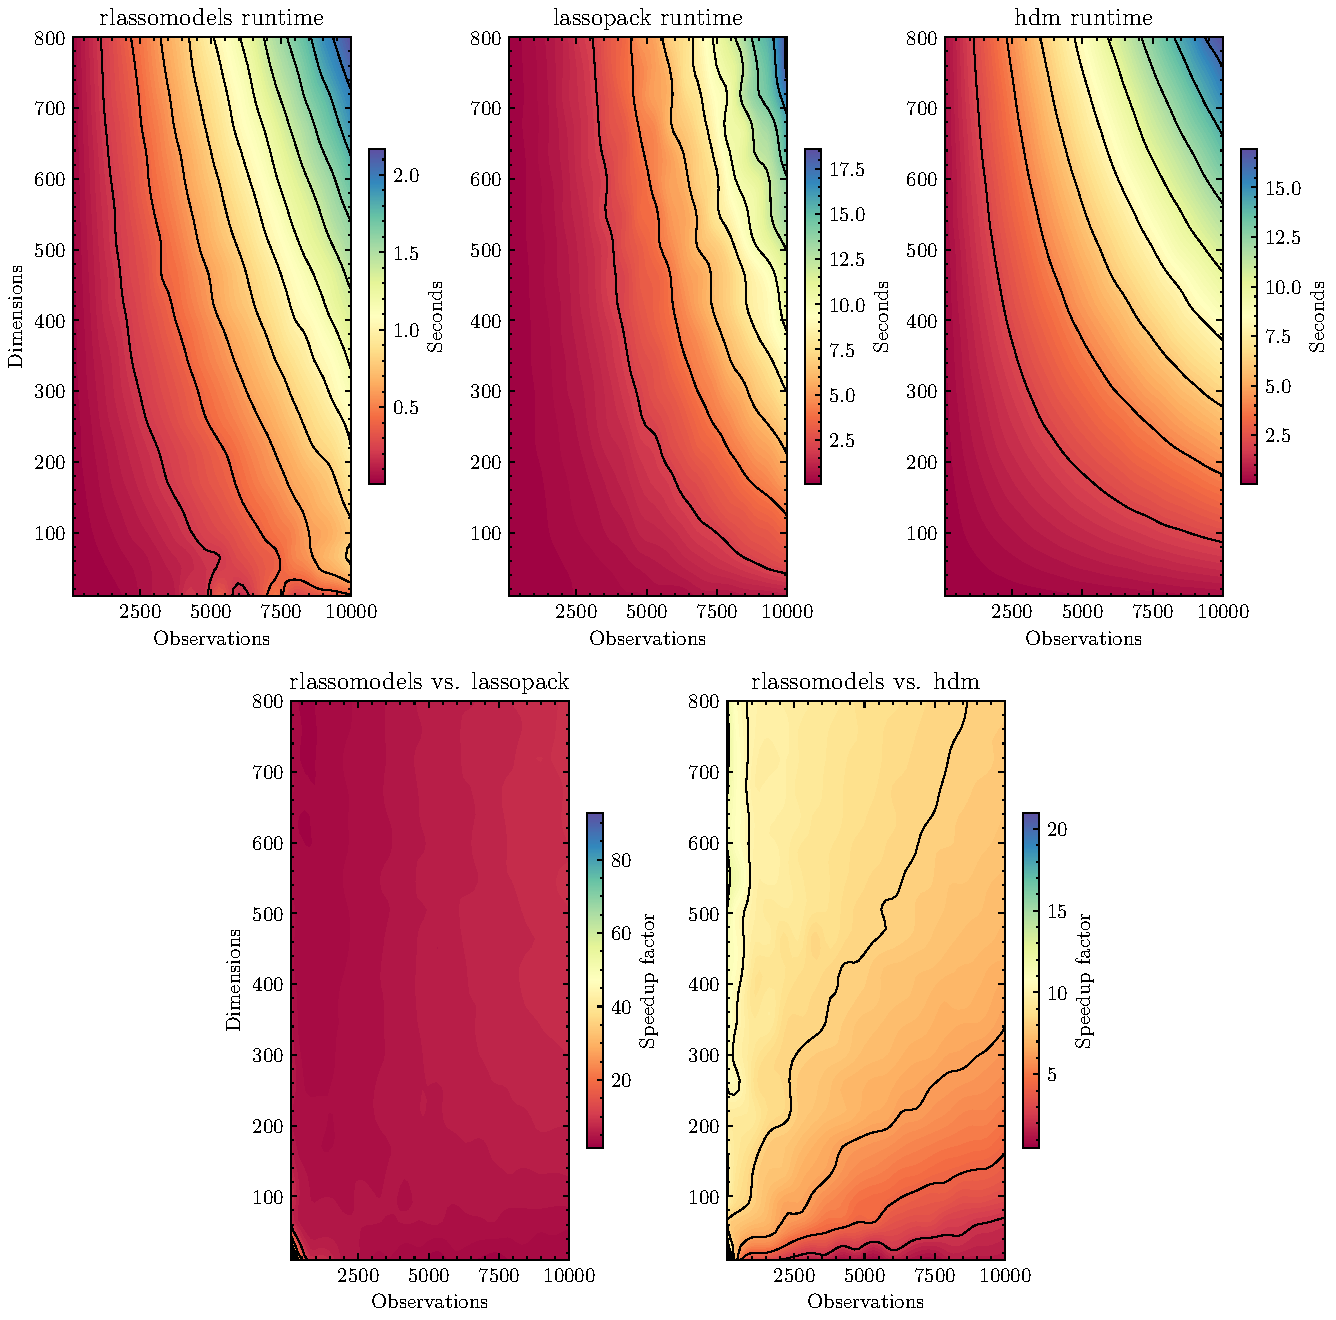
\includegraphics[width=\textwidth]{../outputs/figs/runtime-benchmark.pdf}
  \caption{The figure shows finite sample performance of rigorous lasso and
    other common alternatives in terms of relative empirical risk and F1 score.}
  \label{fig:rlasso-performance}
\end{figure}


\section{Monte-Carlo Examples}

This section aims to highlight some of the finite sample properties of the
rigorous lasso estimator that make it suitable for inferential research. The
results are not new and the Monte-Carlo examples have already been displayed of
several papers. As such, the section is intended as a proof of concept of the
implementation 

\subsection{Rigorous Lasso and post-lasso} As a first step we analyze the
performance of the rigorous choice of penalty level and penalty loadings
relative to other common alternatives. Specifically, we consider the
cross-validation method (CV), the Akaike information criterion (AIC) and the
Bayesian information criterion (BIC). Data is generated the same way as inj
Section \ref{sec:benchmarks}, using the Toeplitz matrix, but with fixed $p =
\dim(x_i) = 200$, $n=100$ and the true support given by $\beta_j = \mathbbm{1}\{j
\leq 5\}$. The DGP linking $x_i$ to $y_i$ is linear with a stochastic noise
term drawn from $\epsilon_i \sim N(0, 1)$, for which we vary $\sigma$ between $0.1$
and $3.5$. For each value of $\sigma$, $100$ simulations are repeated and three
performance metrics computed. Following \cite{Belloni2011}, we compute the
relative empirical risk of each estimator by 

\begin{equation}
\label{eq:empirical risk}
\hat{\delta} = \frac{ \frac{1}{R} \sum_{r=1}^{R} \lVert \tilde{\beta_{r}} -
\beta_0 \rVert_2 }
{\frac{1}{R} \sum_{r=1}^{R} \lVert {\beta_{r}^{*}} -
\beta_0 \rVert_2 }
\end{equation}

\noindent where $\beta^*$ is the oracle estimator, defined as running ordinary
least squares on the regressors set with the true support and $\tilde{\beta}$
is the estimator under consideration. Secondly, the root-mean-squared error is
computed. Lastly, the F1 score is computed to assess how well the estimator
performs model selection by considering both the number of false positives and
false negatives. The simulation results are summarized in Figure
\ref{fig:rlasso-performance} and more details are given in Table
\ref{tab:rlasso-performance}. From the first plot we can see that normal
rigorous lasso is outperformed by CV, AIC and BIC. However, when doing
post-lasso OLS, it achieves near oracle performance for $\sigma < 2$. This
result is understandable from looking at the second plot which shows that
rigorous lasso performs close to perfect model selection for the same values of
$\sigma$. In contrast, CV and AIC perform poorly in terms of F1 as they are
overfitting to the data and selecting too many coefficients.


\begin{figure}[h]
  \centering
  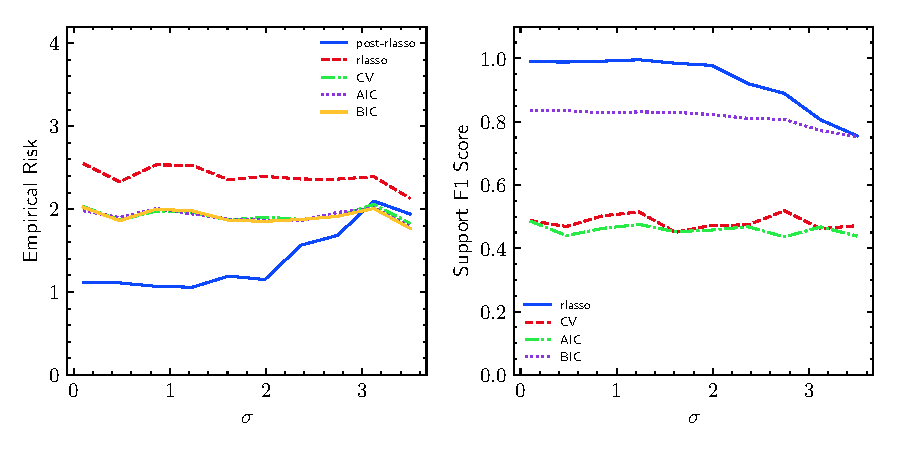
\includegraphics[width=\textwidth]{../outputs/figs/rlasso-oracle.pdf}
  \caption{The figure shows finite sample performance of rigorous lasso and
    other common alternatives in terms of relative empirical risk and F1 score.}
  \label{fig:rlasso-performance}
\end{figure}

\subsection{Inferential properties}

We now move away from the prediction performance of rigorous lasso and focus on
the performance of the post-double-selection and post-partialing out estimators
when the goal is inference.


\section{Empirical Examples}

\section*{Appendix A. Optimization Details}

\section*{Appendix B. Penalty Loadings}

\section*{Appendix C. Further Monte-Carlo Experiments}

\bibliographystyle{ecta}
\bibliography{/Users/matiaspiqueras/Library/texmf/bibtex/bib/Zotero}

\end{document}
